
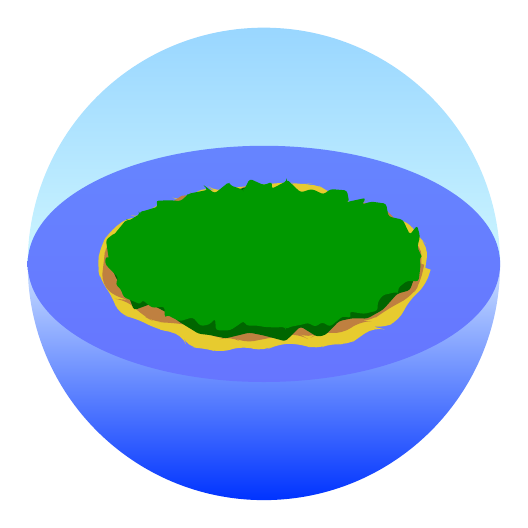
\begin{tikzpicture}
    \def\rayon {3}
    \def\vertical {1.3}

 %\shade[bottom color=blue!40!brown!40!, top color=cyan!20!]
 %\draw (0,0) circle (5cm);

\shade[bottom color=blue!20!cyan!20!, top color=blue!40!cyan!40!]
  (-\rayon,0) arc (180:0:\rayon) -- (-\rayon,0); % CIEL

\shade[bottom color=cyan!20!blue, top color=blue!60!cyan!20!]
  (-\rayon,0) arc (180:360:\rayon) -- (-\rayon,0); % MER

\shade[bottom color=cyan!10!blue!60!, top color=cyan!20!blue!60!]
 (0,0) ellipse (3 and 1.5); % MER

%\shade[bottom color=green!20!brown!60!, top color=brown, decoration={random steps, segment length=2mm}, decorate] (0,0) ellipse (2 and 1); % TERRE
\fill[color=yellow!60!brown, decoration={random steps, segment length=2mm}, decorate, rounded corners]
 (0,-0.05) ellipse (2.05 and 1.05); % SABLE
\fill[color=brown, decoration={random steps, segment length=2mm}, decorate, rounded corners] (0,0.0) ellipse (2 and 0.95); % TERRE


  \fill [green!40!black, decoration={random steps, segment length=2mm}, decorate, rounded corners=1pt]
(0,0) ellipse (1.9 and 0.9); % SOUS VÉGÉTATION
  \fill [green!60!black, decoration={random steps, segment length=1mm}, decorate, rounded corners=1pt](0,0.1) ellipse (2 and 0.9); % SUR VÉGÉTATION

%  \fill [green!70!black, decoration={random steps, segment length=1mm}, decorate](0,0.2) ellipse (0.6 and 0.3);

 % \fill [green!\f!black, decoration={random steps, segment length=0.4mm}, decorate](0,0) ellipse (\n *2 and \n);
 % \fill [green!\f!black, decoration={random steps, segment length=0.4mm}, decorate](0,0) ellipse (\n *2 and \n);


%\draw (-\rayon,0) arc (180:0:\rayon);



%(x0,y0) arc (angledébut:anglefin:rayon)

\end{tikzpicture}


%%%%%%%%%%%%%%%%%%%%%%%%%%%%%%%%%%%%%%%%%%%



